\section{Overall Structure}\label{sec:overall}

\begin{figure}
  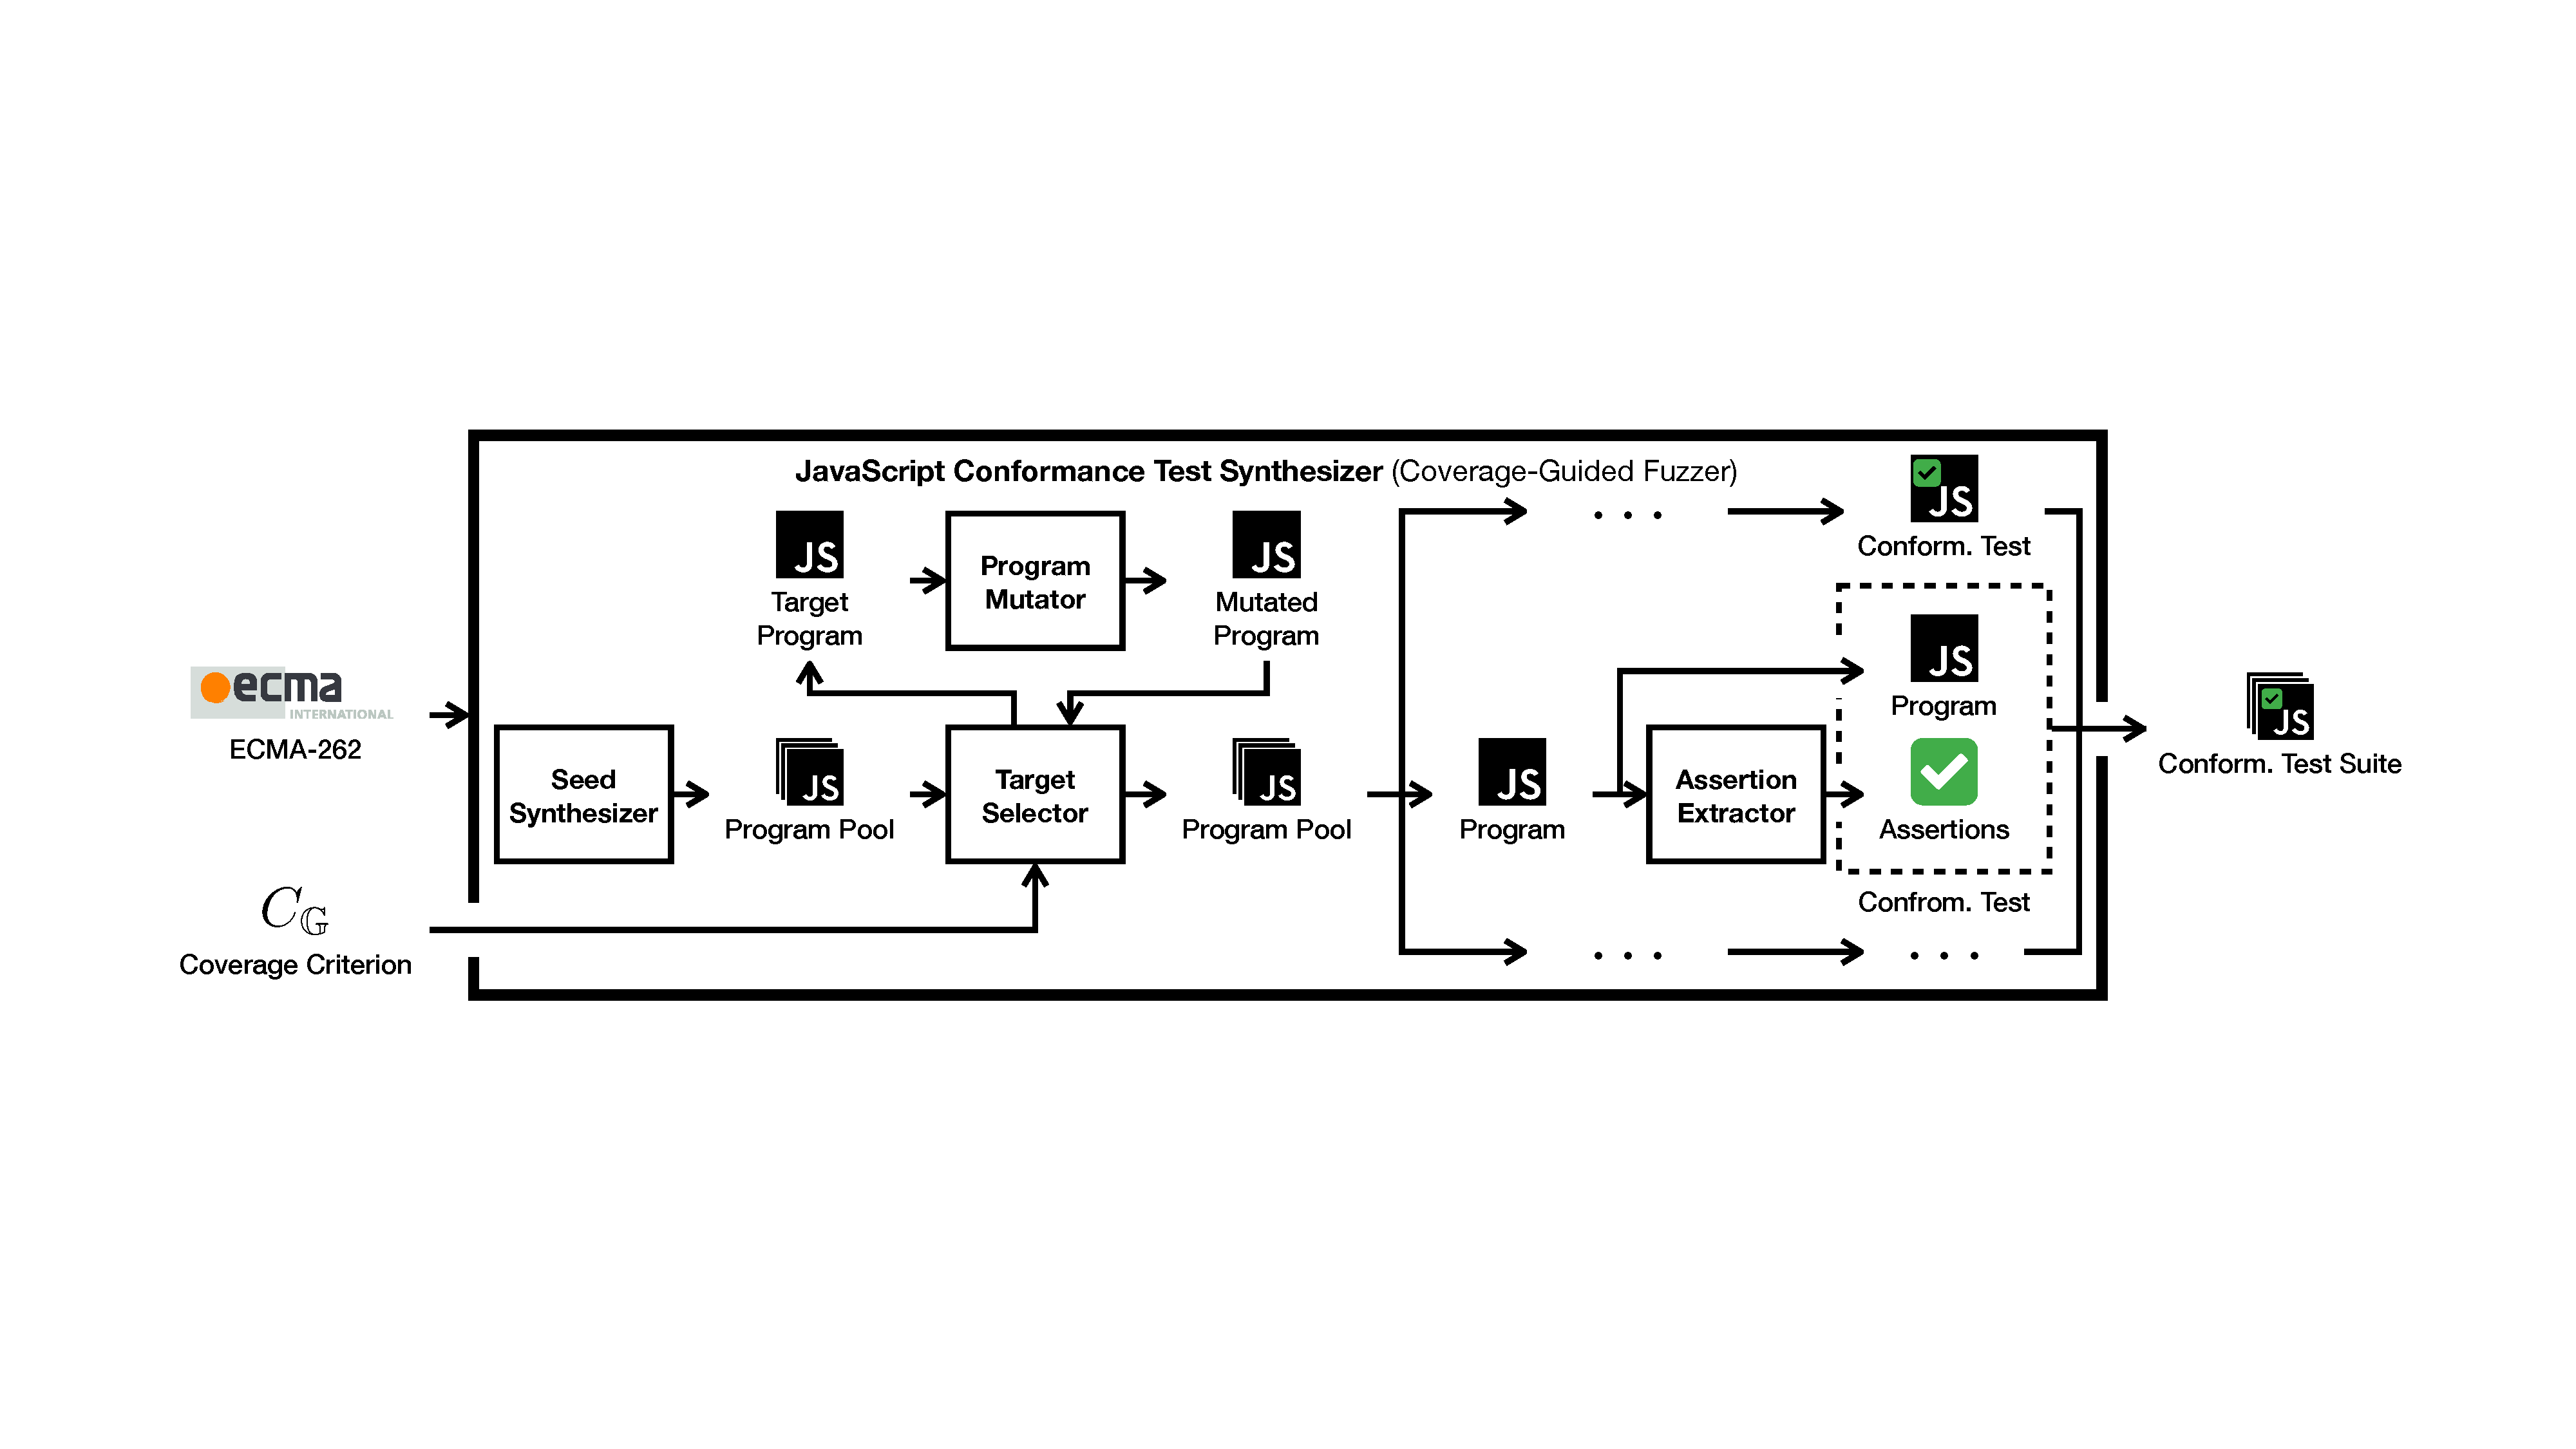
\includegraphics[width=\textwidth]{img/overall}
  \caption{
    Overall structure of a JavaScript conformance test synthesizer using
    coverage-guided fuzzing with CFG in the language specification, ECMA-262.
  }
  \label{fig:overall}
\end{figure}

%----------------------------------------%

This section explains the overall structure of a conformance synthesizer using
coverage-guided fuzzing~\cite{afl} with CFG in the language specification.
%
As depicted in Figure~\ref{fig:overall}, it takes 1) ECMA-262, the JavaScript
official language specification, and 2) a coverage criterion $\cov{\graph}$ for
CFG in the specification.
%
It consists of four different modules that utilize JavaScript syntax and
semantics described in the given language specification:
\begin{itemize}
  \item \textsf{Seed Synthesizer}: As the first step, it automatically
    synthesizes a set of JavaScript programs as the initial \textit{program
    pool}.
    %
    It utilizes JavaScript syntax described in the language specification to
    cover diverse alternatives in syntactic productions as much as possible.
  \item \textsf{Target Selector}:
    It measures the coverage in the CFG based on the given coverage criterion
    $\cov{\graph}$ by interpreting each program in the pool using the abstract
    algorithms in the specification.
    %
    If a program does not cover new TRs, it removes the program from the pool.
    %
    Then, it selects a program as a mutation target in the pool that potentially
    increases the coverage or stops the iteration when the current status
    satisfies the termination condition.
  \item \textsf{Program Mutator}:
    It repeatedly tries to mutate a given JavaScript program to a new one based
    on mutation strategies.
    %
    It is possible to use multiple mutation strategies, and the speed of
    coverage increase is highly dependent on mutation strategies.
  \item \textsf{Assertion Extractor}:
    After the mutation iteration, it automatically extracts assertions of each
    program in the pool.
    %
    The assertions represent the expected final state of each program according
    to the semantics described in the specification.
    %
    As a result, each pair of a program and the corresponding extracted
    assertions is a \textit{conformance test} for JavaScript.
\end{itemize}

%----------------------------------------%

\begin{figure}
  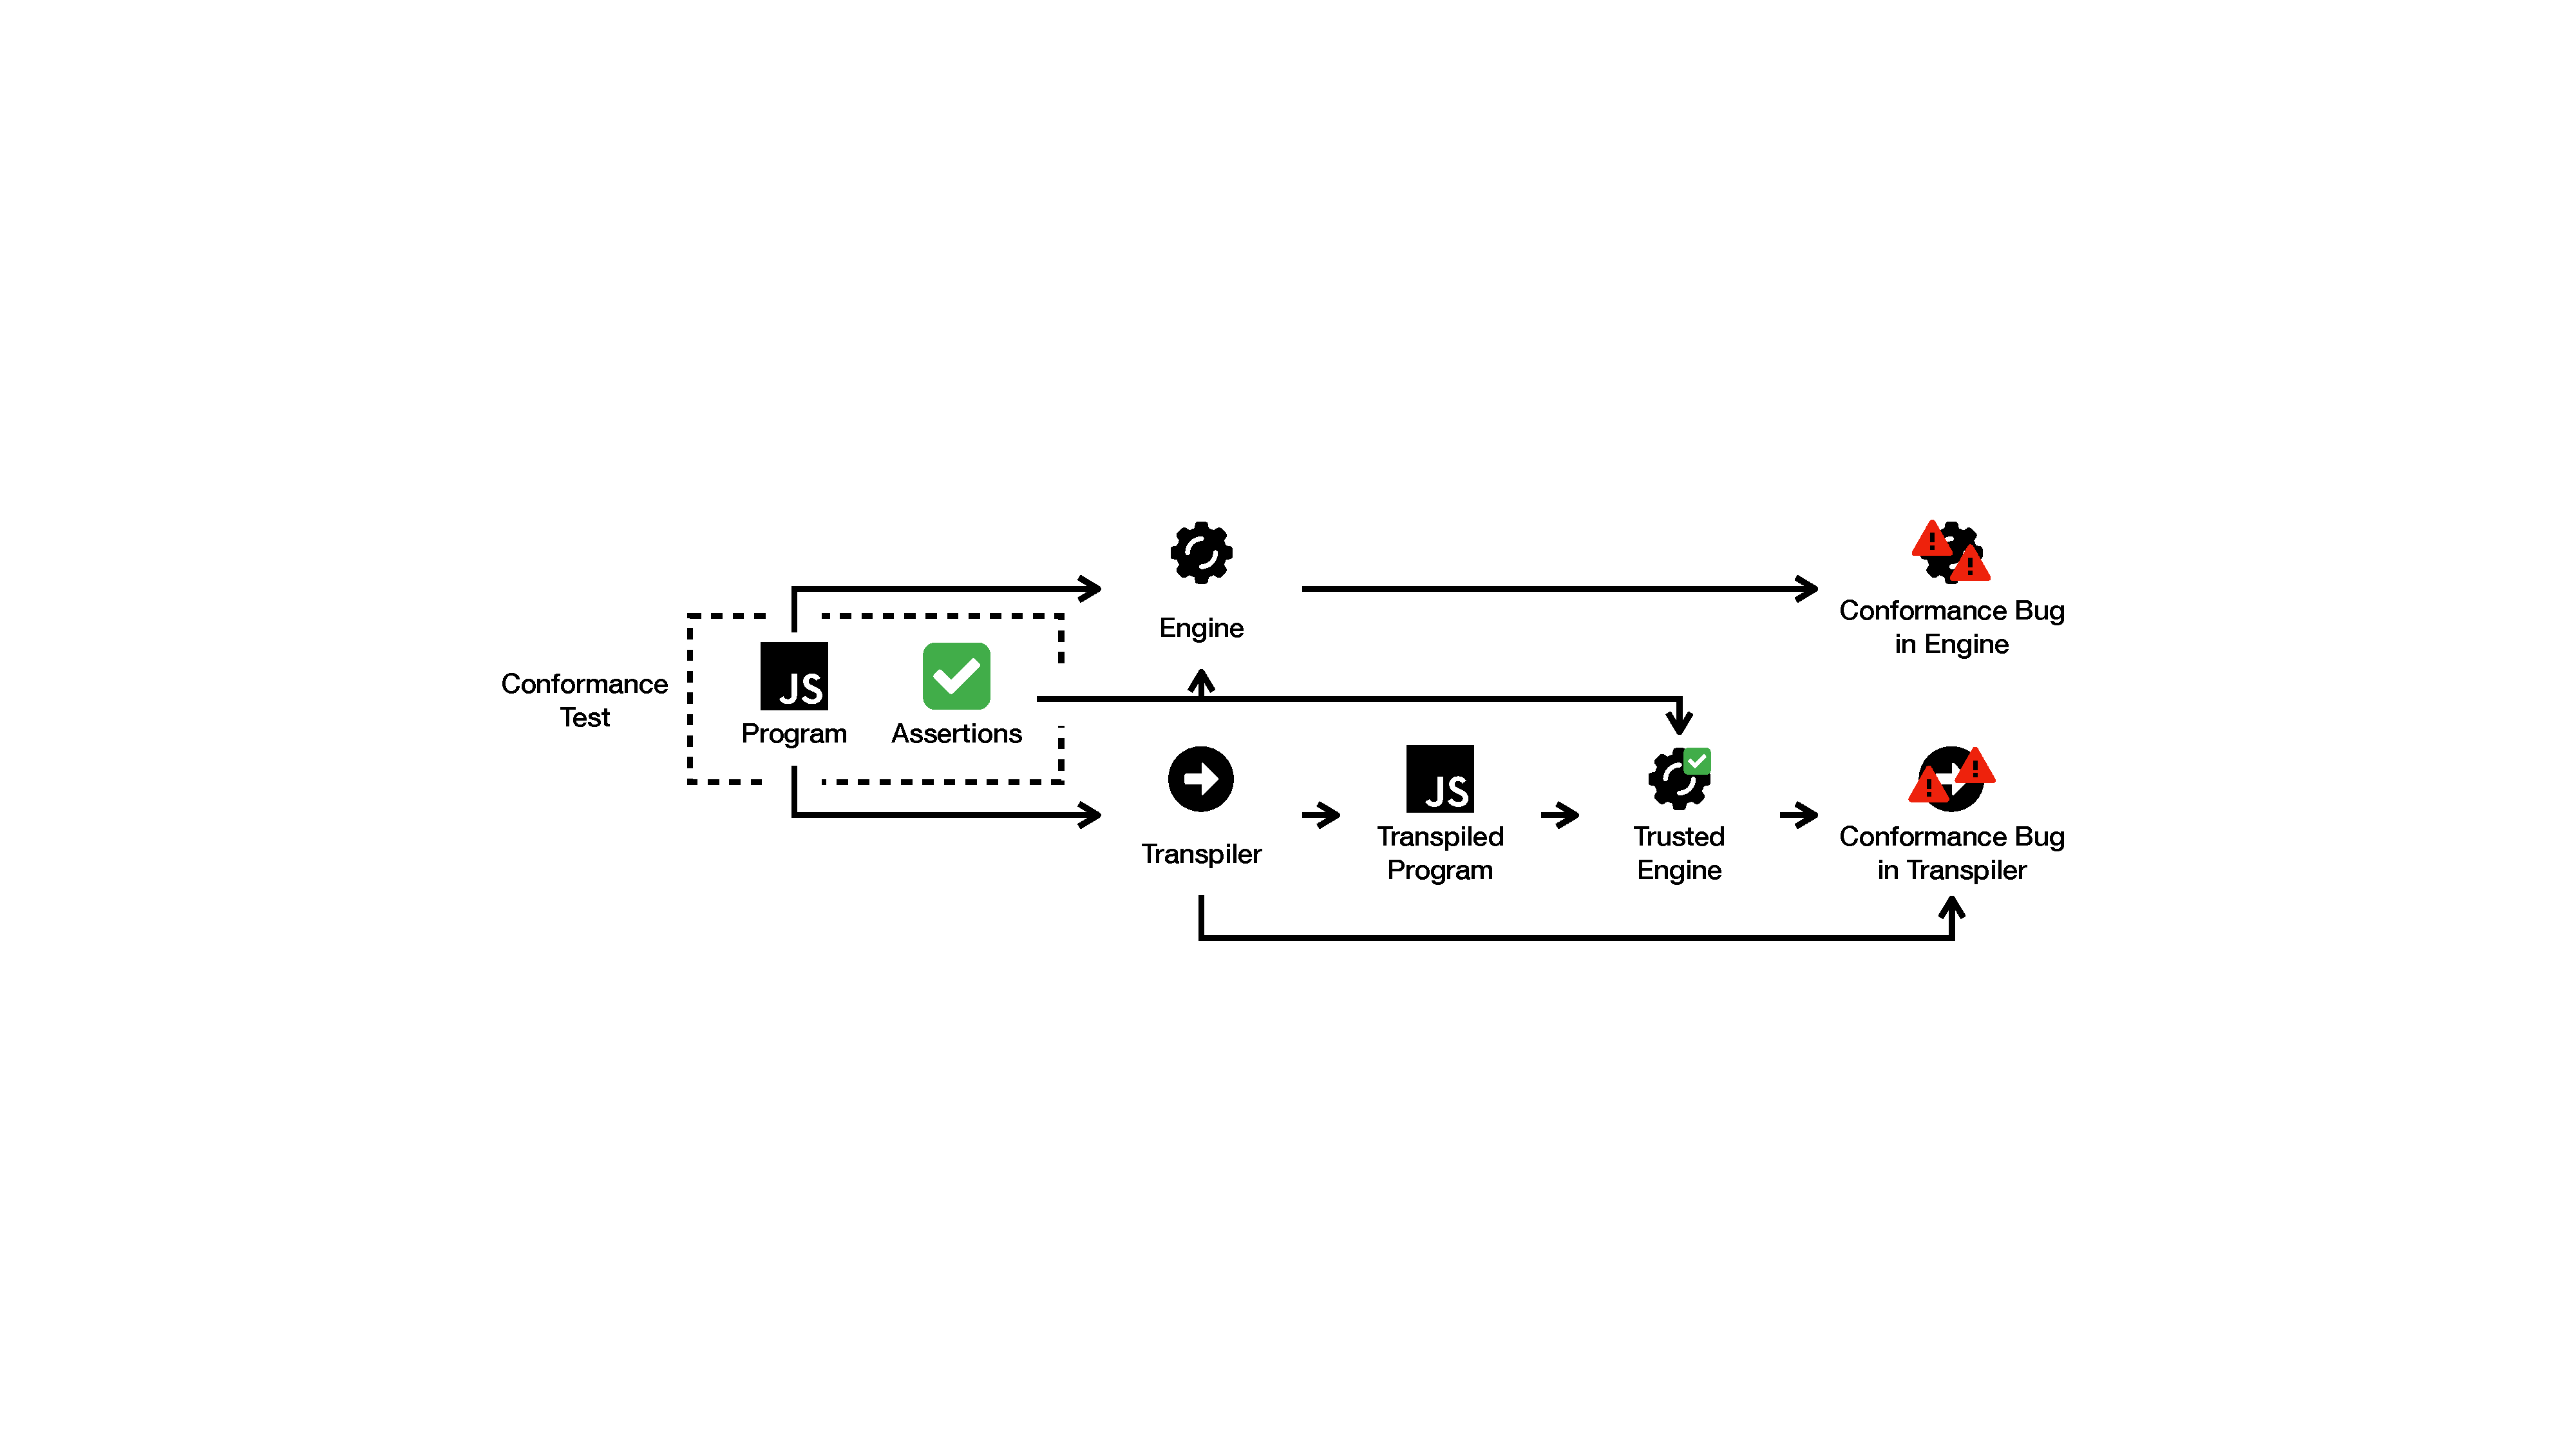
\includegraphics[width=0.8\textwidth]{img/conform-check}
  \caption{
    Conformance check of both engines and transpilers with synthesized
    conformance tests.
  }
  \label{fig:conform-check}
\end{figure}

%----------------------------------------%

\paragraph{\textbf{Conformance Check of Engines and Transpilers}}
%
A synthesized conformance test consists of a JavaScript program and
corresponding assertions.
%
Figure~\ref{fig:conform-check} depicts how to use it to check the conformance of
JavaScript engines and transpilers.
%
First, assume that we want to check the conformance of a JavaScript engine.
%
In this case, it is enough to run the program and assertions together in the
target engine.
%
If an assertion fails, we know the target engine has a conformance bug related
to the test.
%
On the other hand, for JavaScript transpilers, we need to transpile the program
first and run the transpiled program and assertions together using an engine.
%
Note that a trusted or already tested JavaScript engine is required to correctly
check the conformance of transpiler.
